\chapter{Simulation Environment}
\section{Introduction}
small scale helicopters are highly nonlinear system with complex coupling. Analyzing velocity fields around rotor require complicated experiments and numerical methods, which differs in each flight regimes such as hover, stall etc. \cite{doerffer2008numerical,crittenden2004combustion,patterson1990computational}. There are numerous studies on mathematical models of the helicopter dynamics and governing equations of the forces and moments applied to it.
are described in \cite{padfield2008helicopter,marques2017advanced, seddon2011basic}. For this study we have used the model already developed for Evolution-EX helicopter in \cite{pourrezaei2014control}. Here we briefly discuss the model development of this helicopter.
\section{Governing equations}
The Evolution-EX helicopter's (EEH) dynamics are described by a combination of four subsystems: the rigid-body dynamics of the fuselage, the main rotor, the tail rotor, and the empennage. Like other dynamic problems, 2 frameworks are defined, the body (B) and the Inertia (I)  framework. 
\subsection{States and control input}
The states regarding the UAV dynamics include the velocity vector $[3\times1]$:
\begin{equation}
	V=[u,v,w]^T	
\end{equation}
and the angular velocity vector $[3\times1]$:
\begin{equation}
	\omega=[p,q,r]^T
\end{equation}
with respect to {B} and 
the position vector $[3\times1]$:
\begin{equation}
	p=[x,y,z]^T
\end{equation}
and the Euler angles vector $[3\times1]$:
\begin{equation}
	\Theta=[\phi,\theta,\psi]^T
\end{equation}
with respect to {I}
and the input vector $[4\times1]$:
\begin{equation}
	U=[\delta_{col},\delta_{lat},\delta_{lon},\delta_{ped}]^T
\end{equation} 
In the next section the governing equations regarding the states are discussed

\subsection{State-space equations}
The Newton-Euler equations of motion of the helicopter fuselage are defined as:
\begin{equation}\label{eq1}
	\dot{V}=\frac{1}{m} F-\omega\times V
\end{equation}
\begin{equation}\label{eq2}
	\dot{\omega}=I^{-1}M-I^{-1}(\omega \times I \omega) 
\end{equation}
\begin{equation}
	\dot{\Theta}=\Phi(\Theta)\omega 
\end{equation}
\begin{equation}
	\dot{p}=R_{b}^N(\Theta)V
\end{equation}
F and M are defined as vector of external forces and moments respectively. Derivation of F and M are elaborated in \ref{force section} and \ref{Moment section} respectively. $R_b^I$ and $\Phi$ are linear and angular velocity transformation matrices given as follows: 
\begin{gather}
	R_b^I
	=
	\begin{bmatrix}
		s(\theta)c(\psi) &
		-c(\phi)sin(\psi)+s(\phi)s(\theta)c(\psi)&
		s(\phi)s(\psi)+c(\phi)s(\theta)c(\psi) \\
		c(\theta)s(\psi) &
		c(\phi)c(\psi)+s(\phi)s(\theta)s(\psi)&
		-s(\phi)c(\psi)+c(\phi)s(\theta)s(\psi)\\
		-s(\theta)&
		s(\phi)c(\theta)&
		c(\phi)c(\theta)
	\end{bmatrix}
\end{gather}
\begin{gather}
	\Phi
	=
	\begin{bmatrix}
		1 &
		s(\phi)t(\theta)&
		c(\phi)t(\theta) \\
		0 &
		c(\phi)&
		-s(\phi)\\
		0&
		\frac{s(\phi)}{c(\theta)} &
		\frac{c(\phi)}{c(\theta)}
	\end{bmatrix}
\end{gather}
in which s, c and t stands for "sin", "cos" and "tan" respectively.
The I is the moment of inertia in which the off-diagonal terms are neglected:
\begin{equation}
	I=
	\begin{bmatrix}
		I_{xx} &
		0&
		0 \\
		0 &
		I_{yy}&
		0\\
		0&
		0&
		I_{zz}
	\end{bmatrix}
\end{equation}
In the next sections, equations regarding the derivation of forces and moments in \ref{eq1} and \ref{eq2} are introduced.
\subsection{blade flapping}
The dynamics of main rotor-stabilizer bar of the EEH is modeled by \textit{hybrid model approach} \cite{mettler2002system}. In this approach $\dot{a}$ and $\dot{b}$ are  tip-path-plane (TPP) longitudinal and lateral flapping angles respectively and the coefficients of first harmonic approximation in the Fourier series form. The rotor flapping state equations are:
\begin{equation}
	\dot{a}=-q-\frac{a}{\tau_{f}}+\frac{1}{\tau_{f}}(K_u\mu_x+K_w\mu_z)+\frac{A_{lon}}{\tau_{f}} (\delta_{lon}+K_c c)+A_b\frac{b}{\tau_{f}}
\end{equation}
\begin{equation}
	\dot{b} = -p-\frac{b}{\tau_{f}}+\frac{1}{\tau_{f}}(K_v\mu_y)+\frac{B_{lat}}{\tau_{f}}(\delta_{lat}+K_d d)+B_a \frac{a}{\tau_{f}}
\end{equation}
In which $\mu_x,\mu_y$ and $\mu_z $ are the non-dimensional airflow components defined as:
\begin{equation}
	\begin{aligned}
		\mu_x&=\frac{u-u_{wind}}{\Omega R_{mr}}\\
		\mu_y&=\frac{v-v_{wind}}{\Omega R_{mr}} \\
		\mu_z&= \frac{w-w_{wind}}{\Omega R_{mr}}\\
	\end{aligned}
\end{equation}
And the $K_{u}$, $K_v$ and $K_w$ are given by:
\begin{equation}
	K_{u}=2K_{\mu}(\frac{4}{3}\delta_{col}-\frac{Vi}{\omega R_{mr}})
\end{equation}
\begin{equation}
	K_v=-K_u
\end{equation}
\begin{equation}
	K_w=16K_{\mu} \mu_{mr}^2 \frac{sign(\mu_{mr})}{(1-\mu_{mr}^2/2)*(8sign(\mu_{mr})+CL_\alpha \sigma)}
\end{equation}
The stabilizer bar state equations c and d are TPP longitudinal and lateral flapping angles of the stabilizer bar given by:
\begin{equation}
	\dot{c}=-q-\frac{c}{\tau_s}+\frac{C_{lon}}{\tau_s}\delta_{lon}
\end{equation}
\begin{equation}
	\dot{d}=-p-\frac{d}{\tau_s}+\frac{D_{lat}}{\tau_s}\delta_{lat}
\end{equation} 
\subsection{Force derivation} \label{force section}
The force is derived as follows:
\begin{equation}
	F= 
	\begin{bmatrix}
		F_x \\
		F_y\\
		F_z\\
	\end{bmatrix}
	+R_b^I \begin{bmatrix}
		0 \\
		0\\
		mg\\
	\end{bmatrix}
\end{equation}
in which:
\begin{equation}
	F_x=-a\ T_{mr}+F_{x,fus}
\end{equation}
\begin{equation}
	F_y=b\ T_{mr}+T_{tr}+F_{y,fus} + F_{y,vt}
\end{equation}
\begin{equation}
	F_z=-T_{mr}+F_{z,fus} + F_{z,ht}
\end{equation}
Main rotor thrust $T_{mr}$ is given by:
\begin{equation}
	T_{mr} = f_{T_{mr}}+b_{T_{mr}}U;
	\label{T_mr}
\end{equation}
in which:
\begin{equation}\label{f_t}
	f_{T_{mr}}= \frac{1}{4} \rho \pi R_{mr}^4\Omega^2\sigma_{mr}(C_{L_{0}}(\frac{2}{3}+\mu_x^2+\mu_y^2)+C_{L_{\alpha}}(\mu_z-\lambda_0))
\end{equation}
$\lambda_0$ is the inflow ratio expressed as:
\begin{equation}
	\lambda_0=\frac{V_i}{\Omega R_{mr}}
\end{equation}
$\sigma_{mr}$ is the solidity factor derived by:
\begin{equation}
	\sigma_{mr}=\frac{Nc_{mr}}{\pi R_{mr}}
\end{equation}
and $b_{T_{mr}}$ in \ref{T_mr} is control input coefficient term given by:
\begin{equation}\label{b_T}
	b_{T_{mr}}= \frac{1}{4} \rho \pi R_{mr}^4 \Omega^2 \sigma_{mr} C_{L_{\alpha}}\begin{bmatrix}
		\mu_x^2+\mu_y^2+\frac{2}{3}&
		-\mu_y&
		\mu_x&
		0
	\end{bmatrix}
\end{equation}
Similarly, it is possible to derive the tail rotor thrust $T_{tr}$
\begin{equation}
	T_{tr} = f_{T_{tr}}+b_{T_{tr}}U;
\end{equation}
In which $f_{T_{tr}}$ is:
\begin{equation}\label{f_t_tr}
	f_{T_{tr}}=- \frac{1}{4} \rho \pi R_{tr}^4 n_{tr}^2\Omega^2\sigma_{tr}C_{L\alpha_{tr}}v_{tail}
\end{equation}
and input coefficients $b_{T_{tr}}$ is given by:
\begin{equation}\label{b_Ttr}
	b_{T_{tr}}= -\frac{1}{4} \rho \pi R_{tr}^4 n_{tr}^2 \Omega^2 \sigma_{tr} C_{L\alpha_{tr}}\begin{bmatrix}
		0&
		0&
		0&
		u_{tail}^2+w_{tail}^2+\frac{2}{3}
	\end{bmatrix}
\end{equation}
The normalized velocities at tail rotor can be given as:

\begin{equation}
	\begin{aligned}
		u_{tail}&=\frac{u-u_{wind}}{\Omega_{tr} R_{tr} }\\
		v_{tail}&=\frac{v-v_{wind}-V_{i_{tr}}+x_{fus}r}{\Omega_{tr} R_{tr}} \\
		w_{tail}&= \frac{w-w_{wind}-K_{\lambda}V_i+x_{fus}q}{\Omega_{tr} R_{tr}}\\
		\Omega_{tr}&=n_{tr}\Omega  
	\end{aligned}
\end{equation}

$F_{y,vt}$ is the vertical tail force derived by:

\begin{equation}\label{Yvt}
	F_{y,vt}=\frac{1}{2} \rho S_{vt} \Big( C_{L_\alpha}^{vt}V_{vt}(v-v_{wind})+v_{vt}^2 \Big)
\end{equation}

And horizontal tail force $F_{z,ht}$ is:

\begin{equation} \label{Z_ht}
	F_{z,ht}=\frac{1}{2} S_{ht} \Big( C_{L_{\alpha}}^{ht} \mid u-u_{wind} \mid w_{ht} +w_{ht}^2 \Big)    
\end{equation}

In equation \ref{Yvt} $V_vt$ and $v_{tail}$ are axial and normal velocities in vertical tale defined as:

\begin{equation}
	\begin{aligned}
		V_{vt}&=\sqrt{(u-u_{wind})^2+(w- w_{wind} +x_{vt}q-K_\lambda V_i)^2}\\
		v_{tail}&=v-v_{wind}+x_{vt}r-V_{i_{tr}} \\
	\end{aligned}
\end{equation}

Similarly in equation \ref{Z_ht}:

\begin{equation}
	w_{ht}=w-w_{wind}-x_{ht}q-K_{\lambda}V_i
\end{equation} 

$F_{z,fus} , F_{y,fus}$ and $F_{x,fus}$ are drag forces derived by:

\begin{equation}
	F_{x,fus}=-\frac{1}{2} \rho S_x^{fus} V_{fus} (u-u_{wind})
	\label{X_fus}
\end{equation}

\begin{equation}\label{Y_fus}
	F_{y,fus}=-\frac{1}{2} \rho S_y^{fus} V_{fus} (v-v_{wind})
\end{equation}

\begin{equation}\label{Z_fus}
	F_{z,fus}=-\frac{1}{2} \rho S_z^{fus} V_{fus} (w-w_{wind}+V_i)
\end{equation}

the dynamic pressure of the fuselage $V_{fus}$ in expression \ref{X_fus} is defined as:

\begin{equation}
	V_{fus}=\sqrt{(u-u_{wind})^2+(v-v_{wind})^2+(w-w_{wind}+V_i)^2}
\end{equation}

\subsection{Moment derivation} \label{Moment section}

Moment includes 3 terms roll, pitch and yaw:

\begin{equation}
	M =\begin{bmatrix}
		M_{roll}\\
		M_{pitch}\\
		M_{yaw}\\
	\end{bmatrix}
\end{equation}

These three terms are given by:

\begin{equation}
	M_{roll} = (K_{\beta}-T_{mr}Z_{cg})b;%-Ttail*z_fus;
\end{equation}

\begin{equation}
	M_{pitch} = (K_\beta-T_{mr}Z_{cg})a;
\end{equation}

\begin{equation}
	M_{yaw} = Q_{mr}+T_{tr}x_{fus};
\end{equation}
Main rotor drag torque $Q_{mr}$ is derived by:
\begin{equation}
	Q_{mr} = f_{Q_{mr}}+b_{Q_{mr}}U;
\end{equation}
In which:
\begin{equation} \label{f_Q}
	f_{Q_{mr}}=\frac{1}{8} \rho \pi R_{mr}^5 \Omega^2 \sigma_{mr} C_{L_{\alpha}}  \bigg( \frac{C_{D0}}{C_{L_{\alpha}}} \Big( \mu_x^2+\mu_y^2+1 \Big)-2(\mu_{z}-\lambda_0)^2 \bigg)
\end{equation}
\begin{equation} \label{b_Q}
	b_{Q_{mr}}=\frac{1}{8} \rho \pi R_{mr}^5 \Omega^2 \sigma_{mr} C_{L_{\alpha}} (\lambda_0-\mu_z)  \begin{bmatrix}
		\frac{4}{3}
		-\mu_y&
		\mu_x &
		0
	\end{bmatrix}  
\end{equation}

\subsection{induced velocity}

As indicated in \cite{johnson2012helicopter} and \cite{leishman2006principles} the blade element analysis considers each blade
element as a two-dimensional airfoil. The aerodynamic behavior of neighboring
blade elements are independent of each other. An induced inflow velocity on each
blade element should be accounted, which is a product of the rotor wake. Analytical
ways of calculating the induced velocity may be found using momentum theory,
vortex theory or nonuniform inflow calculations \cite{johnson2012helicopter}.\\

In general, the calculation of the inflow velocity is a very challenging task, due to its non-uniformity across the blade span; mathematical simplifications should be applied in order to minimize the complexity of the analysis. Finally, after determining the velocity components
of the blade element, the aerodynamic forces acting on this element are calculated.
The complete dynamic behavior of the blade is obtained by integrating the applied
forces of the individual elements throughout the blade span. Here we use an experimental approach for induced velocity. \\
$V_i$ and $V_{i_{tr}}$ are induced velocity in main rotor and tail rotor respectively. $V_i$ is given by:
\begin{equation}
	V_i=\frac{v_a}{\sqrt{1+\bar{\mu}^2}}
\end{equation}
in which:
\begin{equation}
	V_h=\sqrt{mg/(2\rho \pi R_{mr}^2)}
\end{equation}
\begin{equation}
	\mu=\sqrt{\mu_x^2+\mu_y^2} 
\end{equation}
\begin{equation}
	\bar{\mu}=\frac{\mu}{V_h/(\Omega R_{mr})} 
\end{equation}
\begin{equation}
	V_a=-\frac{w-w_{wind}}{V_h}
\end{equation}
\begin{equation}
	v_a = \left\{
	\begin{array}{ll}
		-\frac{1}{2} V_a-\sqrt{\frac{V_a^2}{4}-1} & \mbox{if } \ V_a 	\leqslant -2 \\
		1-\frac{1}{2} V_a+\frac{25}{12} V_a^2 +\frac{7}{6} V_a^3 & \mbox{if } \ -2<V_a<0 \\
		-\frac{1}{2} V_a+\sqrt{\frac{V_a^2}{4}+1} & \mbox{if } \ V_a	\geqslant 0 \\
	\end{array}
	\right.
	\label{vamr}
\end{equation}
similarly, $V_{i_{tr}}$ is:

\begin{equation}
	V_{i_{tr}}=\frac{v_{a_{tr}}}{\sqrt{1+\overline{\mu_{tr}}^2}}
\end{equation}

in which:

\begin{equation}
	V_{h_{tr}}=\sqrt{f_{F_{y,mr}}/(2\rho \pi R_{tr}^2 x_{fus} )}
\end{equation}

\begin{equation}
	\mu_{tr}=\sqrt{u_{tail}^2+w_{tail}^2} 
\end{equation}

\begin{equation}
	\overline{\mu_{tr}}=\frac{\mu_{tr}}{V_{h_{tr}}/(\Omega R_{tr})} 
\end{equation}

\begin{equation}
	V_{a_{tr}}=-\frac{v-v_{wind}+x_{fus}r}{V_h}
\end{equation}

\begin{equation}
	v_{a_{tr}} = \left\{
	\begin{array}{ll}
		-\frac{1}{2} V_{a_{tr}}-\sqrt{\frac{V_{a_{tr}}^2}{4}-1} & \mbox{if } \ V_{a_{tr}} 	\leqslant -2 \\
		1-\frac{1}{2} V_{a_{tr}}+\frac{25}{12} V_{a_{tr}}^2 +\frac{7}{6} V_{a_{tr}}^3 & \mbox{if } \ -2<V_{a_{tr}}<0 \\
		-\frac{1}{2} V_{a_{tr}}+\sqrt{\frac{V_{a_{tr}}^2}{4}+1} & \mbox{if } \ V_{a_{tr}}	\geqslant 0 \\
	\end{array}
	\right.
	\label{vatr}
\end{equation}

Instead of using equation \ref{vamr} and \ref{vatr}, we use the following approximate functions by regression as they provide a faster calculation time in simulations.:
\begin{equation}
	v'_a = \frac{4.055}{{\left(1.28V_{a}+1.45\right)}^2+1.7}+0.066
\end{equation}

\begin{equation}
	v'_{a_{tr}} = \frac{4.055}{{\left(1.28V_{a_{tr}}+1.45\right)}^2+1.7}+0.066
\end{equation}

figure \ref{fig_va} depicts the two functions $v_a$ and $v'_a$ based on $V_a$.

\begin{figure}
	\begin{center}
		{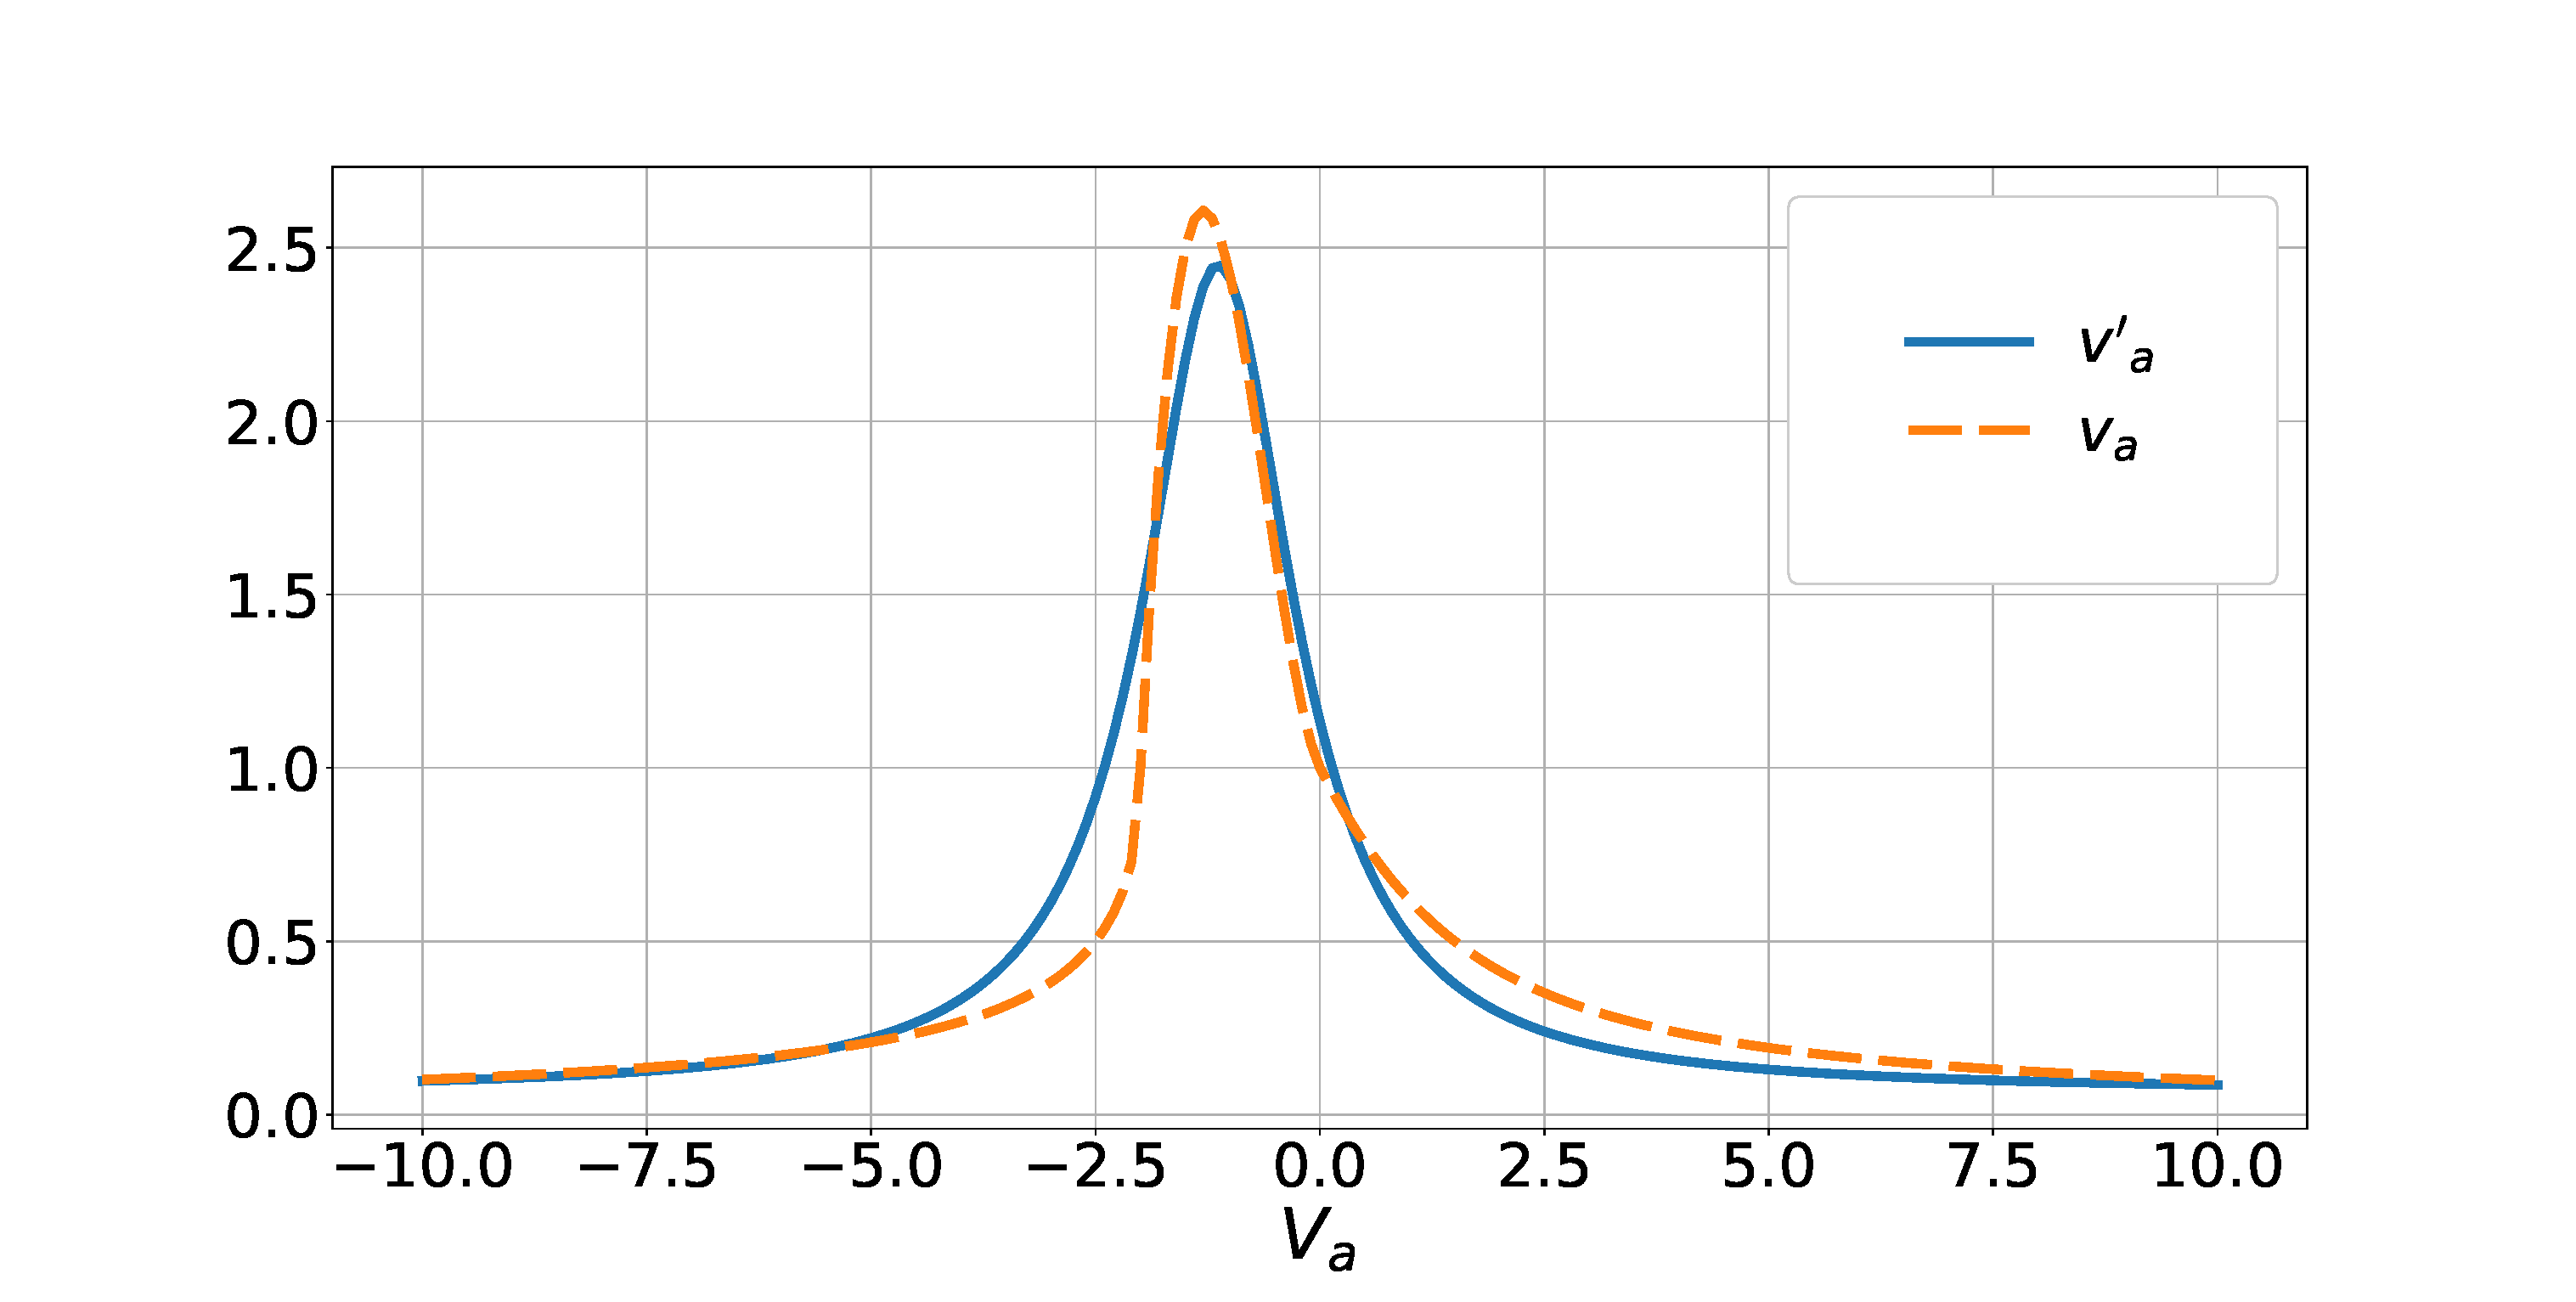
\includegraphics[scale=0.3]{va.eps}}
		
		\caption{function approximation of $v_a$ by $v'_a$, $R^2=0.947$.}
		\label{fig_va}
	\end{center}
\end{figure}
\section{environment setup}

Now that we have discussed the dynamic of the helicopter, it is possible to setup the environment suitable for an RL process, which is developed in OpenAI Gym \cite{brockman2016openai}, which is a software development kit for creating and comparing reinforcement learning algorithms. While trying to implement an RL algorithm in a Gym environment, for each episode first a reset function is called then the step function is called until a terminal state is reached. In the following sections the key points in each part of this environment are discussed. \\

\subsection{reset function} \label{reset}

each time the environment is restarted, the helicopter is randomly placed in a position in which $x$, $y$ and z are uniformly distributed in $[-1,0,1]$ so there would be 27 initial states. Other states are kept constant in this phase at hover state.% !!!!!!!!!!!!!!!!!!!figure

\subsection{step}
In each step of the episode, first the control input is generated from the actions, then RK45 method is used for solving the set of ODEs, In addition, the reward and the condition of reaching a final state is considered. They are elaborated in the upcoming sections.

\subsubsection{Actions}
Instead of having the 4 actions as output of the agent, 16 actions are generated in each step and the control input of the helicopter is find through the following set of equations:

\begin{equation}
	\delta_{col} = a_1 z + a_2 w + a_3
\end{equation} 

\begin{equation}
	\delta_{lat} = a_4 y + a_5 v + a_6 p + a_7 \phi + a_8
\end{equation}

\begin{equation}
	\delta_{lon} = a_9 x + a_{10} v + a_{11} q + a_{12} \theta + a_{13}
\end{equation}

\begin{equation}
	\delta_{ped} = a_{14} r + a_{15} \psi + a_{16}
\end{equation}

This strategy would help the gradient ascent of the agent to more easily find the suitable actions for each step. 

\subsection{Reward}

The reward function is the most important part of the environment as it provides the goal of the RL algorithm. In this research it consists of 5 terms given as follows:

\begin{equation}
	r_t(s) = r_{f} + r_{p} + r_{c} + r_{\psi} + r_u
\end{equation}

\subsubsection{Flying term}

flying reward $r_{f}$ is just a constant (18 in this case) assures that the algorithm is rewarded for longer episodes. Absence of this term will lead to a local minimum of reward in which the agent tries to end the episode to stop receiving negative reward by crashing the helicopter. It also helps to stabilize the UAV in long term. Crashing in this research is when the states are outside of the $[-100,100]$, except for the Euler angles which the bounds are $ \phi \in [-\pi,\pi]$, $ \theta \in [-\pi/2,\pi/2]$ and $ \psi \in [-2\pi,2\pi]$.

\subsubsection{Position term}

the position error $r_{p}$ punishes the agent for the distance between the current position of the UAV and the origin:

\begin{equation}
	r_{p}(t) = 10 \| X(t) \|_2
\end{equation}

\subsubsection{Yaw angle term}

This term is more complicated than the previous ones. If the UAV is headed toward the direction, then it would be easier for it to move toward the origin. For example, if the origin is behind the UAV, the desired $\psi$ would be $-\pi$. Figure  depicts the desired yaw angle $\psi_d$ in x-y plane which is given by:\\

\begin{equation}
	\psi_d=
	\left\{ 
	\begin{array}{ c l }
		-\tan^{-1}(y/x)-\pi/2 & \quad \textrm{if } y \geq0, \quad \quad  \\
		-\tan^{-1}(y/x) +\pi/2    & \quad \textrm{otherwise}, \quad \quad 
	\end{array}
	\right.
\end{equation}

\begin{equation}
	r_\psi = \tanh(x^2+y^2)\min(|\psi-\psi_d|, |\psi-\psi_d+2\pi|,|\psi-\psi_d-2\pi|)
\end{equation}

The $\tanh$ term is added to reduce the effect of this term near the origin, avoiding a sharp change in reward around this area. We have tried to implement the same strategy for $\phi$ and $\theta$, however it did not turn out to be fruitful regarding achieving a better convergence.

\subsubsection{control input terms}

The control input terms consist of a derivative and a norm term to reduce chattering and increase energy consumption of the UAV:
\begin{equation} \label{control_reward}
	r_u = \|U\| + \|U'\| 
\end{equation}

\begin{figure}
	\begin{center}
		\begin{tikzpicture}[scale=3.3,cap=round,>=latex]
			% draw the coordinates
			\draw[->] (-1.5cm,0cm) -- (1.5cm,0cm) node[right,fill=white] {$x$};
			\draw[->] (0cm,-1.5cm) -- (0cm,1.5cm) node[above,fill=white] {$y$};
			
			% draw the unit circle
			\draw[thick] (0cm,0cm) circle(1cm);
			
			\foreach \x in {0,30,...,360} {
				% lines from center to point
				\draw[gray] (0cm,0cm) -- (\x:1cm);
				% dots at each point
				\filldraw[black] (\x:1cm) circle(0.4pt);
				% draw each angle in degrees
				\draw (\x:0.6cm) node[fill=white] {$\x^\circ$};
			}
			
			% draw each angle in radians
			\foreach \x/\xtext in {
				30/,
				45/,
				60/,
				90/,
				120/,
				135/,
				150/,
				180/,
				210/,
				225/,
				240/,
				270/,
				300/,
				315/,
				330/,
				360/}
			\draw (\x:1.25cm) 	node [helicopter top,fill=white,draw=black,minimum width=1cm,rotate=\x+90,scale=0.5] {$$};
			
			% draw the horizontal and vertical coordinates
			% the placement is better this way
			
		\end{tikzpicture}		
	\end{center}
	
	\caption{The desired $\psi$ angle in different orientation in x-y plane.}
	\label{helicopter_psi}
\end{figure}

\subsection{summary}

In this section we provided the dynamics for 6-DOF nonlinear dynamics of a small-scale
UAV, it included the effect of fuselage, main rotor, tail rotor etc. The setup of environment is discussed, and the code is given in Appendix A. The procedure to implement the actions and rewards in this research is also explained in detail. The implementation specifics of the SAC algorithm in this context are elaborated on in the next chapter, and the results are analyzed.  
